\documentclass[12pt,a4paper]{report}
\usepackage[croatian]{babel}
\usepackage[utf8]{inputenc}
\usepackage{amsmath}
\usepackage[margin=3cm]{geometry}
\usepackage{amsfonts}
\usepackage{amssymb}
\usepackage{graphicx}
\usepackage{url}
\usepackage{wrapfig}
%\usepackage{hyperref}

\author{Matea Novak \and Filip Novački \and Ante Vulić}
\title{Linearni splajn. Po dijelovima kubična interpolacija}
\begin{document}
	\maketitle
	
	\tableofcontents
	
\chapter{Uvod}
	Ovo je timski projektni zadatak napravljen je u sklopu kolegija Odabrana poglavlja matematike na Fakultetu organizacije i informatike u Varaždinu Sveučilišta u Zagrebu. Cijeli projekt razvijan je na \texttt{git} repozitoriju koji je dostupan na: \url{https://github.com/filipnovacki/linearni-splajn}. 
\chapter{Zadaci}
	\section{Opis glavne ideje po dijelovima polinomne interpolacije}
	Kod raznih mjerenja, istraživanja i sl. se događa da rezultati nekog testiranja budu podaci koji su diskretni, odnosno izmjereni su za neke vrijednosti. Kako bi nam te vrijednosti bile korisne i primjenjive, moramo na neki način odrediti koje su vrijednosti između dviju diskretnih vrijednosti. Tu u priču dolazi interpolacija.
	
	\begin{wrapfigure}{r}{0.55\textwidth}
		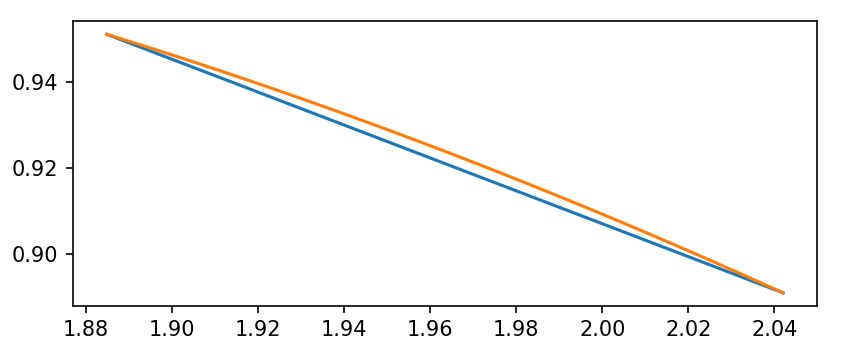
\includegraphics[width=0.55\textwidth]{slike/usporedba.png}
		\caption{Usporedba linearne interpolacije na isječku funkcije $f(x)=\sin x$. Plavom bojom je prikazana interpolacija, a narančastom funkcija. Izvor: autorska izrada}
		\label{usporedba}
	\end{wrapfigure}
	
	Jedna je opcija napraviti interpolaciju linijama prvog reda, dakle, pravcima, odnosno dužinama koje jednostavno povučemo između dviju točaka. Takva aproksimacija je vrlo jednostavna za izračunati, međutim, takvo mjerenje ne daje baš zadovoljavajuće rezultate. Drugi je problem što mjesta gdje se ti pravci spajaju su \textit{oštri}, odnosno ne postoji glatki prijelaz.
	
	Kao što vidimo na slici \ref{usporedba}, plava linija dosta je dosta blizu narančastoj, no za razne primjene bi ta greška mogla biti prevelika.
	
	Bolja opcija je povezati točke krivuljama višeg reda. Kako bismo dobili glatki prijelaz, moramo paziti da derivacija u točkama uvijek bude jednaka. Kvadratični splajn ima jedan nedostatak. Nedostatak je u tome što je zakrivljen uvijek u jednu stranu, odnosno u obliku parabole. Kubična interpolacija je po tom pitanju mnogo bolja jer može imati oblik parabole, ali ne mora. 
	
	Mogu se koristiti i polinomi još višeg reda, međutim oni se nešto teže računaju te funkcije polinoma višeg reda imaju tendenciju na nekim mjestima jako \textit{divljati}, što ponekad može predstavljati problem.
	\section{Opis linearnog splajna}
	
	\section{Primjeri}
		\subsection{Algoritam za traženje linearnog splajna}
		Neka je zadana neprekidna funkcija $f:[a,b]\rightarrow \mathbb{R} $ i neka je segment $[a,b]$ podijeljen na $n$ jednakih dijelova, tj. neka su
		\begin{equation*}
			x_i=a+ih,\quad i=0,1,\ldots,n,\quad h=\frac{b-a}{n}
		\end{equation*}
		
		Algoritam koji računa linearni splajn izmađu dvaju ekvidistantnih čvorova $x_i$ započinje pronalaženjem točaka.
		
		\begin{align*}
			y_i&=f(x_i)\\
			y_{i+1}&=f(x_{i+1})\\
			&\downarrow\\
			T_i&(x_i, y_i)\\
			T_{i+1}&(x_{i+1}, y_{i+1})
		\end{align*}
		
		Zatim moramo pronaći pravac koji je razapet između tih dviju točaka. To možemo napraviti po formuli koja je opće poznata:
		\begin{equation}
		y=\biggr{(}\frac{y_{i+1}-y_i}{x_{i+1}-x_i}\biggr{)}(x-x_i)+y_i
		\label{pravac}
		\end{equation}
		
		
		\subsection{$f(x)=\sin x$}
		Ovaj ćemo zadatak riješiti za $i=1, 2,\ldots, 40$. S obzirom da nema nekog smisla pisati za svaki interval pojedinačno, ovaj ćemo zadatak riješiti programskim putem, a ručno ćemo pokazati samo na jednom primjeru. Tablicu s rješenjima možemo vidjeti u tablici \ref{linInterpolTablica}
		\begin{align*}
			f(x)=\sin (x),& \quad x\in [0, 2\pi]\\
			n&=40\\
			a&=0\\
			b&=2\pi\\
		\end{align*}
		Pronađimo prva dva čvora.
		\begin{align*}
			x_0=&0\quad\rightarrow \quad y_0=f(0)=0\\
			x_1=&a+ih\\=&0+1\frac{2\pi-0}{40}\\
				=&0.15707963267948966\\
			y_1=&f\biggr{(}\frac{2\pi}{40}\biggr{)}\\=&0.15707963267948966
		\end{align*}
		Uvrštavanjem ovih podataka u jednadžbu \ref{pravac} dobivamo:
		\begin{equation}
			y=1.0041242039539873x
			\label{linInt1}
		\end{equation}
		Kad razmislimo o rješenju, vidimo da ono ima smisla jer prolazi kroz ishodište, a nagib je skoro jednak 1, što također ima smisla jer koordinate točke skoro jednake. Osim toga, i grafički rješenje ima smisla, što možemo vidjeti na slici \ref{linInterSlika1}.
		\begin{figure}[h]
			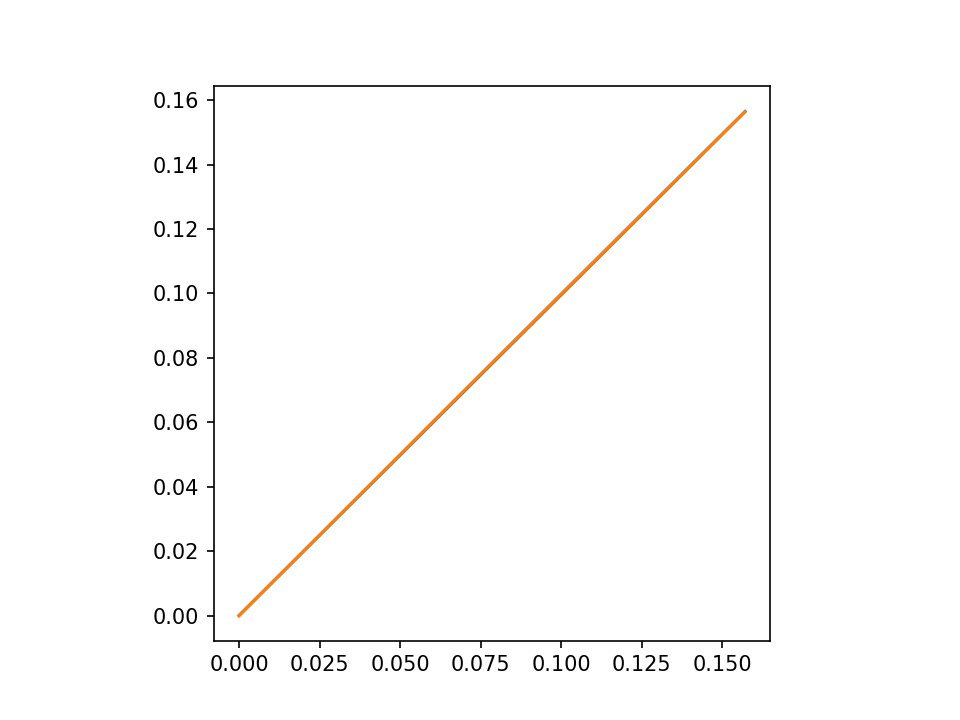
\includegraphics[width=\textwidth]{slike/usporedba40.png}
			\caption{Usporedba funkcije $f(x)=\sin (x)$ i linearne interpolacije po jednadžbi pravca iz jednadžbe \ref{linInt1}. Plavom bojom je prikazana interpolacija, a narančastom funkcija. Izvor: autorska izrada}
			\label{linInterSlika1}
		\end{figure}
		\begin{table}
		\begin{tabular}{c | c c | c c | c | c}
			$i$&$x_1$&$y_1$&$x_2$&$y_2$&Interpolacija&$\text{Razlika}$\\\hline
1 &$0.0000$&$0.0000$&$0.1571$&$0.1564$&$y =  0.9959x+0.0000$&$-0.84$\\
2 &$0.1571$&$0.1564$&$0.3142$&$0.3090$&$y =  0.9714x+0.0039$&$-0.69$\\
3 &$0.3142$&$0.3090$&$0.4712$&$0.4540$&$y =  0.9229x+0.0191$&$-0.53$\\
4 &$0.4712$&$0.4540$&$0.6283$&$0.5878$&$y =  0.8518x+0.0526$&$-0.39$\\
5 &$0.6283$&$0.5878$&$0.7854$&$0.7071$&$y =  0.7596x+0.1105$&$-0.25$\\
6 &$0.7854$&$0.7071$&$0.9425$&$0.8090$&$y =  0.6488x+0.1976$&$-0.13$\\
7 &$0.9425$&$0.8090$&$1.0996$&$0.8910$&$y =  0.5220x+0.3171$&$-0.03$\\
8 &$1.0996$&$0.8910$&$1.2566$&$0.9511$&$y =  0.3823x+0.4707$&$0.05$\\
9 &$1.2566$&$0.9511$&$1.4137$&$0.9877$&$y =  0.2332x+0.6580$&$0.11$\\
10 &$1.4137$&$0.9877$&$1.5708$&$1.0000$&$y =  0.0784x+0.8769$&$0.15$\\
11 &$1.5708$&$1.0000$&$1.7279$&$0.9877$&$y = -0.0784x+1.1231$&$0.16$\\
12 &$1.7279$&$0.9877$&$1.8850$&$0.9511$&$y = -0.2332x+1.3906$&$0.15$\\
13 &$1.8850$&$0.9511$&$2.0420$&$0.8910$&$y = -0.3823x+1.6717$&$0.11$\\
14 &$2.0420$&$0.8910$&$2.1991$&$0.8090$&$y = -0.5220x+1.9569$&$0.05$\\
15 &$2.1991$&$0.8090$&$2.3562$&$0.7071$&$y = -0.6488x+2.2358$&$-0.03$\\
16 &$2.3562$&$0.7071$&$2.5133$&$0.5878$&$y = -0.7596x+2.4969$&$-0.13$\\
17 &$2.5133$&$0.5878$&$2.6704$&$0.4540$&$y = -0.8518x+2.7285$&$-0.25$\\
18 &$2.6704$&$0.4540$&$2.8274$&$0.3090$&$y = -0.9229x+2.9185$&$-0.39$\\
19 &$2.8274$&$0.3090$&$2.9845$&$0.1564$&$y = -0.9714x+3.0555$&$-0.53$\\
20 &$2.9845$&$0.1564$&$3.1416$&$0.0000$&$y = -0.9959x+3.1287$&$-0.69$\\
21 &$3.1416$&$0.0000$&$3.2987$&$-0.1564$&$y = -0.9959x+3.1287$&$-0.84$\\
22 &$3.2987$&$-0.1564$&$3.4558$&$-0.3090$&$y = -0.9714x+3.0478$&$-1.00$\\
23 &$3.4558$&$-0.3090$&$3.6128$&$-0.4540$&$y = -0.9229x+2.8804$&$-1.15$\\
24 &$3.6128$&$-0.4540$&$3.7699$&$-0.5878$&$y = -0.8518x+2.6233$&$-1.30$\\
25 &$3.7699$&$-0.5878$&$3.9270$&$-0.7071$&$y = -0.7596x+2.2759$&$-1.43$\\
26 &$3.9270$&$-0.7071$&$4.0841$&$-0.8090$&$y = -0.6488x+1.8406$&$-1.55$\\
27 &$4.0841$&$-0.8090$&$4.2412$&$-0.8910$&$y = -0.5220x+1.3227$&$-1.65$\\
28 &$4.2412$&$-0.8910$&$4.3982$&$-0.9511$&$y = -0.3823x+0.7303$&$-1.73$\\
29 &$4.3982$&$-0.9511$&$4.5553$&$-0.9877$&$y = -0.2332x+0.0746$&$-1.79$\\
30 &$4.5553$&$-0.9877$&$4.7124$&$-1.0000$&$y = -0.0784x-0.6307$&$-1.83$\\
31 &$4.7124$&$-1.0000$&$4.8695$&$-0.9877$&$y =  0.0784x-1.3693$&$-1.84$\\
32 &$4.8695$&$-0.9877$&$5.0265$&$-0.9511$&$y =  0.2332x-2.1233$&$-1.83$\\
33 &$5.0265$&$-0.9511$&$5.1836$&$-0.8910$&$y =  0.3823x-2.8727$&$-1.79$\\
34 &$5.1836$&$-0.8910$&$5.3407$&$-0.8090$&$y =  0.5220x-3.5967$&$-1.73$\\
35 &$5.3407$&$-0.8090$&$5.4978$&$-0.7071$&$y =  0.6488x-4.2740$&$-1.65$\\
36 &$5.4978$&$-0.7071$&$5.6549$&$-0.5878$&$y =  0.7596x-4.8834$&$-1.55$\\
37 &$5.6549$&$-0.5878$&$5.8119$&$-0.4540$&$y =  0.8518x-5.4044$&$-1.43$\\
38 &$5.8119$&$-0.4540$&$5.9690$&$-0.3090$&$y =  0.9229x-5.8180$&$-1.30$\\
39 &$5.9690$&$-0.3090$&$6.1261$&$-0.1564$&$y =  0.9714x-6.1072$&$-1.15$\\
40 &$6.1261$&$-0.1564$&$6.2832$&$-0.0000$&$y =  0.9959x-6.2574$&$-1.00$\\


			
		\end{tabular}
		\caption{Prikaz svih čvorova funkcije $f(x)=\sin(x)$, jednadžbe pravca koja interpolira između dviju susjednih točaka te razlika između vrijednosti funkcije u točki $x=1$ i interpolacije u istoj točki. U izračunu je korišten maksimalni broj decimala koliko podržava tip podataka \texttt{float} iz \texttt{Python} biblioteke \texttt{Numpy}. Izvor: autorska izrada}
		\label{linInterpolTablica}
		\end{table}
		\subsection{$g(x)=\frac{1}{x^2 +1}$}
	\section{Opis nedostataka linearnih splajnova}
	\section{Opis po dijelovima kubične interpolacije}
	\section{Primjeri}
		\subsection{Algoritam za traženje po dijelovima kubične interpolacije}
		\subsection{$f(x)=\sin x$}
		\subsection{$g(x)=\frac{1}{x^2 +1}$}
\chapter{Zaključak}
\end{document}